\documentclass[11pt,a4paper]{article}
\usepackage[margin=2.2cm]{geometry}
\usepackage[T1]{fontenc}
\usepackage{lmodern}
\usepackage{graphicx}
\usepackage{booktabs}
\usepackage{longtable}
\usepackage{array}
\usepackage{xcolor}
\usepackage{enumitem}
\usepackage{fancyhdr}
\usepackage{float}
\usepackage{titlesec}
\usepackage[hidelinks]{hyperref}

\definecolor{accent}{HTML}{1F4E79}
\definecolor{sevhigh}{HTML}{B03A2E}
\definecolor{sevmed}{HTML}{CA6F1E}
\definecolor{sevlow}{HTML}{1E8449}
\hypersetup{colorlinks=true, linkcolor=accent, urlcolor=accent}
\titleformat{\section}{\Large\bfseries\color{accent}}{\thesection}{0.8em}{}
\titleformat{\subsection}{\large\bfseries\color{accent}}{\thesubsection}{0.6em}{}

\pagestyle{fancy}
\fancyhf{}
\fancyhead[L]{\small OsdagBridge --- Software Testing Report}
\fancyhead[R]{\small dev @ \texttt{d74f56d}}
\fancyfoot[C]{\small Page \thepage}
\renewcommand{\headrulewidth}{0.4pt}

\newcommand{\issue}[1]{\href{https://github.com/Nidhikhare12/OsdagBridge/issues/#1}{\##1}}
\newcommand{\proof}[1]{\texttt{proofs/#1}}
\newcommand{\sevH}{\textcolor{sevhigh}{\textbf{S1}}}
\newcommand{\sevM}{\textcolor{sevmed}{\textbf{S2}}}
\newcommand{\sevL}{\textcolor{sevlow}{\textbf{S3}}}
\newcolumntype{L}[1]{>{\raggedright\arraybackslash}p{#1}}

\begin{document}

% ------------------------------------------------------------------ title
\begin{titlepage}
\centering
\vspace*{2.5cm}
{\color{accent}\rule{\linewidth}{1.2pt}}\\[0.8cm]
{\Huge\bfseries Software Testing Report}\\[0.4cm]
{\LARGE Short-Span Steel Plate Girder Bridge Module\\[0.2cm] of OsdagBridge}\\[0.8cm]
{\color{accent}\rule{\linewidth}{1.2pt}}\\[1.5cm]
{\large FOSSEE Winter Internship --- Screening Task, IIT Bombay}\\[2.2cm]
\begin{tabular}{@{}ll@{}}
\toprule
Software under test & OsdagBridge, branch \texttt{dev}, commit \texttt{d74f56d} \\
Upstream repository & \url{https://github.com/Nidhikhare12/OsdagBridge} \\
Evidence repository & \url{https://github.com/amit-sarkar-svg/osdagbridge-testing-report} \\
Tester (GitHub account) & \texttt{amit-sarkar-svg} \\
Test period & 15 -- 22 November 2026 \\
Report version & 2.1 (22 November 2026) \\
\bottomrule
\end{tabular}
\vfill
{\small All testing was performed on a local, read-only clone of OsdagBridge. No source file of the project was modified; every script, input file, log and screenshot referenced in this report is stored in the evidence repository.}
\end{titlepage}

\tableofcontents
\newpage

% ------------------------------------------------------------------ 1
\section{Executive summary}

The plate girder bridge module of OsdagBridge was tested through its validators, layout solver, \texttt{.osi} loader, full design pipeline, PDF report generator, desktop input dock (run offscreen), command-line entry point and packaging metadata. Static security tooling was applied to the complete source tree.

\begin{center}
\begin{tabular}{@{}lr@{}}
\toprule
Metric & Value \\
\midrule
GitHub issues filed by the tester & \textbf{28} (\issue{96}--\issue{155}, \issue{206}--\issue{213}, \issue{215}, \issue{216}) \\
\quad of which filed in this version (22 Nov 2026) & 5 (\issue{211} \sevH, \issue{212}, \issue{213}, \issue{215}, \issue{216}) \\
\quad filed in version 2.0 (21 Nov 2026) & 5 (\issue{206}, \issue{207}, \issue{208}, \issue{209}, \issue{210}) \\
Root-cause analyses contributed to existing issues & 7 (incl.\ \issue{135}, \issue{88}, \issue{20}, \issue{19}, \issue{42}) \\
Extreme-value cases (validators, layout, loader) & 1\,966, all oracles satisfied \\
Full design runs executed in this version & see Section~\ref{sec:coverage} \\
Issues screened for duplicates (open and closed) & 210 issues, 80 PRs \\
\bottomrule
\end{tabular}
\end{center}

\paragraph{Most significant findings.}
\begin{enumerate}[nosep]
  \item \issue{211} --- the design live load is taken from static vehicles parked at the left support ($x = 0$), never at mid-span. On a 40\,m span the design moment rises by 16.4\,\% when the vehicles are centred; the girder live-load moment is underestimated (unconservative).
  \item \issue{134} --- a valid input combination silently skips the live load, so every design demand is zero and the design is reported as PASS (wrong engineering result).
  \item \issue{135} --- a second \texttt{design()} on the same object crashes. This version identifies the root cause: girder dimensions are converted from mm to m \emph{in place}, so the second run divides them by 1000 again (Section~\ref{sec:contrib}).
  \item \issue{208} --- design-log warnings and errors are collected for the report but never written to it.
  \item \issue{206} / \issue{207} --- clearing an input field silently substitutes a wrong value: skew becomes $-15^\circ$, and the carriageway minimum ignores ``Median = No''.
  \item \issue{215} --- cross-bracing design forces are read from the horizontal component Vz, so dead and live load contribute exactly zero; the members are sized for 1--3\,kN of seismic/wind force.\\ \issue{213} --- the bearing-zone web-buckling check reports a capacity 69 times the squash load; \issue{212} --- a failed report compilation returns an older PDF as the new report.
  \item \issue{96}, \issue{129}, \issue{130}, \issue{88} --- validation gaps: out-of-range or non-finite values reach the design pipeline.
\end{enumerate}

% ------------------------------------------------------------------ 2
\section{Scope and objectives}
\begin{itemize}[nosep]
  \item Verify that documented input limits are enforced consistently by the UI, the validators and the \texttt{.osi} loader.
  \item Exercise the design pipeline headlessly with boundary, combination, custom-material and malformed inputs, and check the results against invariants.
  \item Check state handling across repeated design runs, and agreement between input dictionary, output dictionary, output dock and PDF report.
  \item Review the code for security weaknesses (shell and LaTeX injection, unsafe deserialisation, path handling).
  \item Report only reproducible, evidenced defects, each checked against all existing issues first.
\end{itemize}
\textbf{Out of scope:} the web application (the \texttt{web/} folder contains stubs only, see \issue{155}) and modules other than the plate girder bridge.

% ------------------------------------------------------------------ 3
\section{Test environment}
\begin{tabular}{@{}ll@{}}
\toprule
Operating system & macOS 13.6 (Darwin 22.6.0), Intel, 8 logical CPUs \\
Python environment & Miniconda, env \texttt{osdagbridge-env}, Python 3.12, PySide6 6.11 \\
OsdagBridge & branch \texttt{dev}, commit \texttt{d74f56d}, installed editable \\
LaTeX & TeX Live \texttt{pdflatex} (for report generation) \\
Test tooling & pytest, hypothesis, psutil, bandit, ruff, pip-audit \\
GUI testing & real \texttt{CustomWindow}/\texttt{InputDock} under \texttt{QT\_QPA\_PLATFORM=offscreen} \\
\bottomrule
\end{tabular}

% ------------------------------------------------------------------ 4
\section{Methodology}
\subsection{Ground rules}
\begin{itemize}[nosep]
  \item The OsdagBridge clone is read-only. Proposed fixes are proven by applying them to a \emph{copy} of the function inside the test (monkeypatching).
  \item Each test case runs in its own subprocess with a timeout (600\,s for design, 120\,s for parsers). This means one hang or crash cannot affect other cases.
  \item A defect is \emph{confirmed} only when it has an exact saved input, an expectation with a stated justification, the executed result, and two reproductions in separate fresh processes.
\end{itemize}

\subsection{Classification}
\begin{tabular}{@{}lL{12.5cm}@{}}
\toprule
Tier & Meaning \\
\midrule
T1 & Confirmed: reproduced twice in fresh processes \\
T2 & Likely: executed once or by a narrower path \\
T3 & Static finding: by reading only \\
T4 & Duplicate of an existing issue (extra evidence is posted as a comment) \\
T5 / T6 & Installation or environment blocker / documentation or wording \\
T7 & Oddity that may be intended \\
T8 & Checked and correct \\
T9 & Could not be tested (reason stated) \\
\midrule
\sevH & Wrong engineering result, data loss or security weakness \\
\sevM & Crash or wrong behaviour with a workaround \\
\sevL & Cosmetic or low-impact robustness \\
\bottomrule
\end{tabular}

\subsection{Duplicate screening}
All issues and pull requests of the upstream repository (open and closed) were downloaded with the GitHub CLI (\texttt{notes/issues\_raw.json}). Every candidate was searched against titles \emph{and} bodies with \texttt{scripts/search\_issues.py}. Each issue draft lists the search terms used and the issues they matched.

% ------------------------------------------------------------------ 5
\section{Test coverage and results}\label{sec:coverage}
\begin{longtable}{@{}L{1.0cm}L{4.4cm}L{5.4cm}L{5.4cm}@{}}
\toprule
Layer & Area & Executed & Outcome \\
\midrule
\endhead
L1 & Validators (every key) & 1\,233 cases: limit neighbours, NaN/inf, text forms, types, Unicode digits & All oracles satisfied; NaN gap is the known \issue{88} \\
L2 & Layout solver grid & 33 cases: span, carriageway, skew, footpath, median & All invariants satisfied \\
L3 & \texttt{.osi} loader and parser hazards & 700 cases incl.\ alias bomb, deep nesting, BOM, YAML 1.1 booleans & No crash or hang; gaps are the known \issue{96}, \issue{131}, \issue{153}, \issue{154} \\
L4 & Design pipeline, corner sweep & 16 of 32 corner designs (span 20/45 m, carriageway min/23.6 m, skew $\pm$15$^\circ$, footpath, median): 13 ok, 3 timeout (timeouts are not yet conclusive, see Section~\ref{sec:limits})%
 & No NaN/inf, negative dimension or out-of-range $\chi_{LT}$ in any completed output \\
L5 & Repeated runs and state & Second \texttt{design()} on one object; UI path repeated twice & Crash \issue{135} reproduced and root-caused; UI path stable \\
L6 & PDF report & 8 free-text and file-name cases, end-to-end log check, \LaTeX\ unavailable & \issue{208}, \issue{210}, \issue{212}; LaTeX injection attempt correctly escaped \\
L7 & Desktop input dock (offscreen) & 27 typed-input checks on span, skew and carriageway; empty-field checks & \issue{206}, \issue{207}; non-numeric typing correctly blocked \\
H & Hand calculations and physics oracles & Moving load on 20--40\,m spans (IRC Class A, 70R); squash-load limit; combination factors & \issue{211} \sevH, \issue{213}; extra evidence for \issue{174}, \issue{104} \\
M & Metamorphic sweeps & Span 20/30/40\,m; carriageway 4.25--7.50\,m in 0.25\,m steps (20 full designs, one process each) & Live-load moment falls from 30 to 40\,m (\issue{211}); lane sweep never gives zero live load (correct) \\
L8 & CLI entry point & 7 invocations (help, missing file, directory, empty file, bad flag) & Stub returns 0 for everything --- known \issue{101} \\
S & Static security review & bandit, ruff, pip-audit, targeted grep & No high-severity finding; Section~\ref{sec:static} \\
\bottomrule
\end{longtable}

% ------------------------------------------------------------------ 6
\section{Summary of issues filed}
\begin{longtable}{@{}L{1.1cm}L{8.6cm}L{2.4cm}L{1.0cm}L{2.2cm}@{}}
\toprule
Issue & Title (abridged) & Category & Tier & Severity \\
\midrule
\endhead
\multicolumn{5}{@{}l}{\textit{Filed 22 November 2026 (this version)}} \\
\issue{211} & Design live load from static vehicles parked at $x = 0$; girder live-load moment underestimated & Analysis & T1 & \sevH \\
\issue{212} & Older PDF returned as the new report when compilation fails & Report & T1 & \sevM \\
\issue{213} & Web-buckling check (Cl.\,509.7.3.1) capacity 69$\times$ the squash load; always passes & Design check & T1 & \sevM \\
\issue{215} & Cross-bracing forces read from horizontal Vz: gravity loads contribute 0 & Design & T1 & \sevH\,(cand.) \\
\issue{216} & Cross-bracing report tables: KL/r $\neq$ KL/$r_{min}$, UR $\neq$ D/C & Report & T1 & \sevM \\
\midrule
\multicolumn{5}{@{}l}{\textit{Filed 21 November 2026}} \\
\issue{206} & Clearing the Skew Angle field silently sets skew to $-15^\circ$ instead of $0^\circ$ & Validation / UI & T1 & \sevM \\
\issue{207} & Carriageway validator treats Median = ``No'' as a median (7.5\,m instead of 4.25\,m) & Validation & T1 & \sevM \\
\issue{208} & Design-log warnings and errors never written to the PDF report & Report & T1 & \sevM \\
\issue{209} & \texttt{\_lookup\_material} returns \texttt{None} / raises \texttt{IndexError} & Robustness & T1 & \sevL \\
\issue{210} & \texttt{\_tex()} double-escapes backslashes (prints ``\textbackslash\{\}'') & Report & T1 & \sevL \\
\midrule
\multicolumn{5}{@{}l}{\textit{Filed 15 -- 18 November 2026}} \\
\issue{96} & \texttt{.osi} loading skips all custom-material validation & Validation & T1 & \sevM \\
\issue{97} & Input lock can crash if Additional Inputs was never opened & UI state & T3 & \sevM \\
\issue{98} & \texttt{osdag\_core} metadata declares bogus \texttt{sqlite} dependency & Install & T5 & \sevM \\
\issue{99} & \texttt{pyproject.toml} omits required runtime dependencies & Install & T5 & \sevM \\
\issue{100} & Inconsistent dependency declarations across manifests & Packaging & T6 & \sevL \\
\issue{101} & README documents a CLI, but the entry point is a stub & Docs / CLI & T6 & \sevL \\
\issue{127} & Verification example YAMLs are empty placeholders & Docs & T6 & \sevL \\
\issue{128} & \texttt{example\_basic.yaml} passes validation vacuously & Docs & T7 & \sevL \\
\issue{129} & Material validator skips cross-bracing / end-diaphragm ranges & Validation & T2 & \sevM \\
\issue{130} & Integer validators raise \texttt{OverflowError} on \texttt{inf} & Validation & T2 & \sevM \\
\issue{131} & \texttt{saveOSI\_inputs} writes unsafe YAML tags & File I/O & T2 & \sevM \\
\issue{132} & Skew sign is not mirror-symmetric ($+15^\circ$ vs.\ $-15^\circ$) & Analysis & T2 & \sevH \\
\issue{133} & Span 45\,m + median + footpaths: \texttt{design()} does not terminate & Performance & T2 & \sevM \\
\issue{134} & Valid input silently skips live load; design reported PASS & Analysis & T1 & \sevH \\
\issue{135} & Second \texttt{design()} on the same object crashes & Crash / state & T1 & \sevM \\
\issue{153} & \texttt{saveOSI\_inputs} does not enforce the \texttt{.osi} extension & File I/O & T3 & \sevL \\
\issue{154} & \texttt{loadOSI\_inputs} silently swallows exceptions & File I/O & T3 & \sevM \\
\issue{155} & No web application layer (Django/React are stubs) & Scope / docs & T5 & \sevL \\
\bottomrule
\end{longtable}
All issues were open at the time of writing. Severities for \issue{96}--\issue{155} were assigned for this summary from the impact described in each issue.

% ------------------------------------------------------------------ 7
% Findings filed 22 November 2026 (report version 2.1)
\section{Detailed findings filed in this version (22 November 2026)}

These three findings came from a second round aimed at engineering results rather than input handling: hand calculations with the program's own IRC~6 vehicle tables, a span metamorphic test, physics oracles on design-check capacities, and fault injection in report generation. Each was reproduced in two fresh processes. All 210 upstream issues (open and closed) were searched for duplicates first.

% ---- 211
\subsection{\issue{211} --- Design live load taken from vehicles parked at $x = 0$}
\textbf{Severity / tier:} \sevH\ / T1. \quad \textbf{Proof:} \proof{211\_static\_vehicles\_fixed\_at\_x0/}

\textbf{Description.} \texttt{create\_governing\_ll\_load\_case()} (\texttt{analyser.py:1925}) selects the design live load only from the static vehicle cases (filter at line 1951). Every static vehicle is placed with its origin at the left support: \texttt{x\_coord = 0.0} (line 1641), applied at line 1834. The moving-load cases, which do traverse the span (lines 1908--1910), are not used for this selection. On a 40\,m span all static wheel loads lie in $x \in [0.6, 20.3]$\,m (2 $\times$ Class~A) and $[0.81, 13.75]$\,m (70R).

\textbf{Expected:} the live-load effect at the critical vehicle position. For a fixed set of vehicles, the maximum moment on a simply supported span increases with span.

\begin{center}\begin{tabular}{@{}lrrr@{}}
\toprule
40\,m span & Current ($x = 0$) & Vehicles centred & Change \\
\midrule
Governing LL $\max|M_z|$ & 1106.3\,kNm & 1527.7\,kNm & +38\,\% \\
LL moment per girder & 775--797\,kNm & 1362--1389\,kNm & +71--79\,\% \\
Design moment \texttt{mu\_applied} & 3553.9\,kNm & 4137.7\,kNm & +16.4\,\% \\
\bottomrule
\end{tabular}\end{center}

\textbf{Hand calculation.} Moment with the vehicle fixed at $x = 0$ divided by the moment at the worst position, single simply supported line: Class~A 0.89 / 0.90 / 0.84 / 0.71 and 70R 1.00 / 0.92 / 0.84 / 0.71 for spans 20 / 25 / 30 / 40\,m.

\textbf{Metamorphic check.} The program's live-load moment summed over the girders is 2240.4\,kNm (20\,m), 3216.4\,kNm (30\,m) and 3145.2\,kNm (40\,m): it \emph{decreases} from 30 to 40\,m.

\textbf{Fix (proven):} centring the static vehicles on the span (monkeypatch of the x offset only) gives the values in the right-hand column. Selecting the governing LL from the moving-load envelope would also fix it.

\begin{figure}[H]\centering
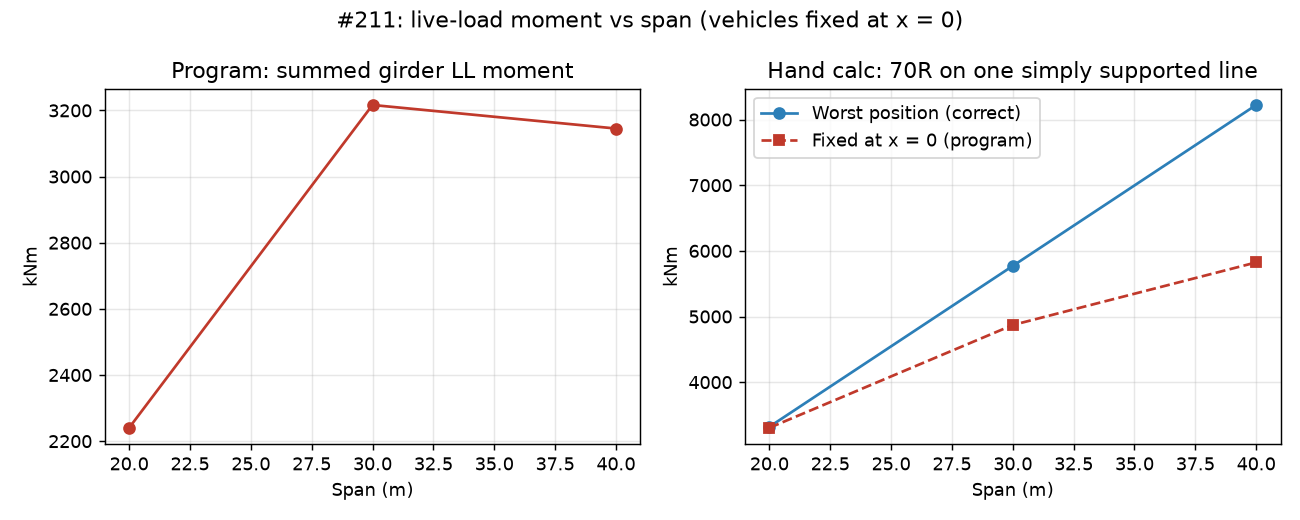
\includegraphics[width=0.92\linewidth]{../proofs/211_static_vehicles_fixed_at_x0/report_output/span_vs_ll_moment.png}
\caption{Left: program live-load moment against span (falls between 30 and 40\,m). Right: hand calculation for 70R, worst position against fixed at $x = 0$.}
\end{figure}

% ---- 212
\subsection{\issue{212} --- Older PDF returned as the new report when compilation fails}
\textbf{Severity / tier:} \sevM\ / T1. \quad \textbf{Proof:} \proof{212\_stale\_pdf\_returned\_as\_success/}

\textbf{Description.} \texttt{generate\_report()} judges success by \texttt{os.path.exists(pdf\_path)} in the output folder (\texttt{report\_generator.py:981--983}). The new PDF is copied there only if it was produced (lines 978--979). When compilation fails, a PDF left by an earlier report passes the check and is returned as the new report.

\textbf{Test.} A report for project PROJECTOLDA was generated normally; a second report for PROJECTNEWB was then generated into the same folder with \texttt{pdflatex} removed from \texttt{PATH} (child process only).

\textbf{Expected:} \texttt{pdf\_path = None} and an error. \quad \textbf{Actual:} \texttt{pdf\_path} returned as success; the PDF is byte-identical to the first one (same SHA-256 and modification time) and still shows PROJECTOLDA, while the new \texttt{.tex} contains PROJECTNEWB. The only trace is a log warning. Reproduced twice.

\textbf{Fix:} remove the old PDF before compiling, and test the PDF produced in the temporary folder together with the \texttt{pdflatex} return code.

\begin{figure}[H]\centering
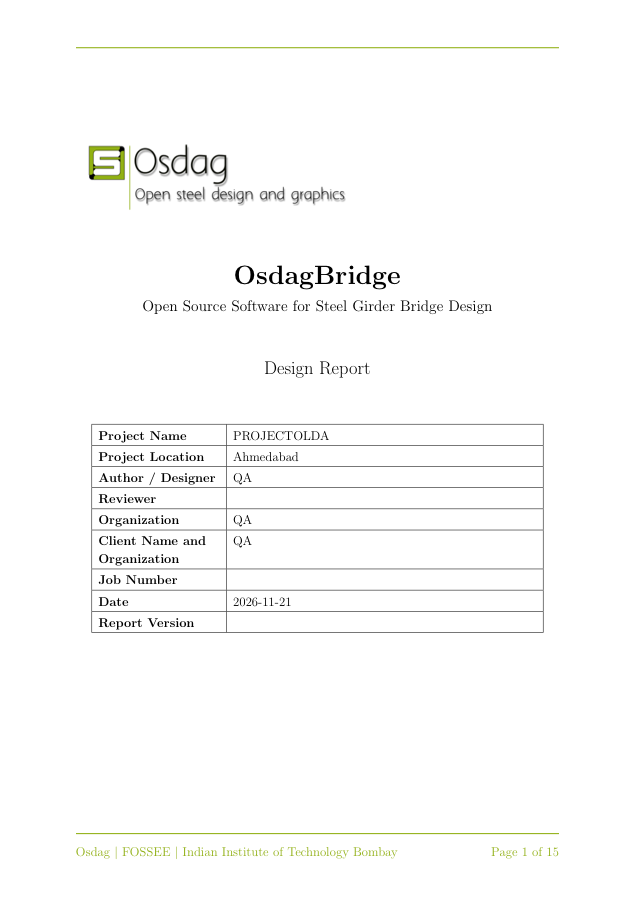
\includegraphics[width=0.36\linewidth]{../proofs/212_stale_pdf_returned_as_success/screenshots/returned_pdf_page1_shows_PROJECTOLDA.png}
\caption{Title page of the PDF returned for project PROJECTNEWB: it still shows PROJECTOLDA.}
\end{figure}

% ---- 213
\subsection{\issue{213} --- Web-buckling capacity 69 times the squash load}
\textbf{Severity / tier:} \sevM\ / T1. \quad \textbf{Proof:} \proof{213\_web\_buckling\_exceeds\_squash\_load/}

\textbf{Description.} The check ``Brg.Stiff: Web Buckling'' (Cl.\,509.7.3.1) is, by its own comment, for the \emph{unstiffened} web bearing zone (\texttt{designer.py:1665}). Lines 1668--1670 compute the radius of gyration from the bearing-stiffener inertia divided by the bare-web area, and use the raw Euler stress $\pi^2 E/(KL/r)^2$ with no yield cap and no buckling curve. The stiffener column check next to it (line 1691) does use the program's design compressive-stress function.

\begin{center}\begin{tabular}{@{}lr@{}}
\toprule
Quantity (span 20\,m case) & Value \\
\midrule
Radius of gyration used (web alone: $t_w/\sqrt{12} = 2.31$\,mm) & 80.1\,mm \\
Reported stress $f_{cc}$ ($f_y = 350$\,MPa) & 21\,858.5\,MPa \\
Reported capacity (demand $R = 250.0$\,kN) & 109\,506\,kN, PASS \\
Squash load $A f_y/\gamma_{m0}$, $A = 5010$\,mm$^2$ & 1\,594\,kN \\
Program's own $f_{cd}$ for the web strut, $KL/r = 331$ & 14.7\,MPa $\Rightarrow$ 73.8\,kN, FAIL \\
\bottomrule
\end{tabular}\end{center}

\textbf{Expected:} a capacity not above the squash load; with the program's own function the unstiffened web fails, consistent with a bearing stiffener being provided. \quad \textbf{Impact:} the value is reported (design-check list and output dictionary) but does not drive another decision, because bearing stiffeners are checked separately. Reproduced twice.

\subsection{Extra evidence for existing issues}
\begin{itemize}[nosep]
  \item \issue{174} (combination factors): for the 20\,m case \texttt{BASIC\_1} (1.35\,DL) and \texttt{BASIC\_4} (1.0\,DL) give the same moment, 1092.872\,kNm; \texttt{mu\_applied} is 1141.8\,kNm against about 1705\,kNm by hand.
  \item \issue{104} (empty reactions table): the data behind the table is also wrong --- for every load case the left reaction equals minus the right, and only interior girders are summed (\texttt{results\_data.py:964--983}).
\end{itemize}


\section{Detailed findings filed 21 November 2026}

% ---- 206
\subsection{\issue{206} --- Clearing the Skew Angle field sets skew to $-15^\circ$}
\textbf{Severity / tier:} \sevM\ / T1. \quad \textbf{Proof:} \proof{206\_empty\_skew\_resets\_to\_minus15/}

\textbf{Description.} When the Skew Angle field is emptied and loses focus, the validator returns \texttt{SKEW\_ANGLE\_MIN} as the ``corrected'' value. The widget and the input dictionary are overwritten with $-15.0$. The popup only says that a numeric value is required. \texttt{SKEW\_ANGLE\_DEFAULT = 0.0} exists (\texttt{common.py:332}) but is never used. Because the skew sign is not mirror-symmetric (\issue{132}), the substituted sign also changes the results.

\textbf{Expected:} 0.0 (the defined default), or the field flagged without being changed. \quad \textbf{Actual:} $-15.0$ in the widget and in \texttt{input\_dict}.

\textbf{Root cause:} \texttt{validator.py:63--64}, \texttt{return SKEW\_ANGLE\_MIN, "Skew angle must be a numeric value."}

\textbf{Fix (proven):} return \texttt{SKEW\_ANGLE\_DEFAULT}. With this patch the empty-field result is 0.0.

\begin{figure}[H]\centering
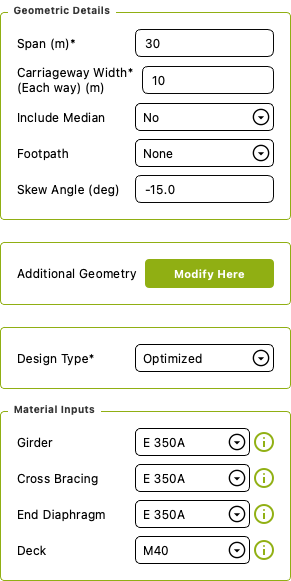
\includegraphics[width=0.30\linewidth]{../proofs/206_empty_skew_resets_to_minus15/screenshots/02_after_clearing_skew.png}
\caption{Input dock (offscreen capture) after the Skew Angle field, previously 5, was cleared: it now shows $-15.0$.}
\end{figure}

% ---- 207
\subsection{\issue{207} --- Median = ``No'' treated as a median by the carriageway validator}
\textbf{Severity / tier:} \sevM\ / T1. \quad \textbf{Proof:} \proof{207\_median\_no\_treated\_as\_yes/}

\textbf{Description.} The carriageway branch of \texttt{validate\_basic\_inputs} tests the median flag in two inconsistent ways: \texttt{if median} at line 46, and \texttt{median == 'Yes'} at line 49. The UI stores the strings ``No'' and ``Yes'', and ``No'' is truthy. With Median = No and no width, the with-median minimum of 7.5\,m is suggested instead of 4.25\,m.

\begin{center}\begin{tabular}{@{}lll@{}}
\toprule
\texttt{include\_median} & Returned minimum & Correct? \\
\midrule
\texttt{"Yes"} & 7.5 & yes \\
\texttt{"No"} & 7.5 & \textbf{no} (4.25 expected) \\
\texttt{""} / \texttt{None} & 4.25 & yes \\
\bottomrule
\end{tabular}\end{center}

\textbf{Root cause:} \texttt{validator.py:46}. \quad \textbf{Fix (proven):} \texttt{if median == 'Yes' else}. A copy of the method with this change returns 4.25 for ``No'' and 7.5 for ``Yes''.

\begin{figure}[H]\centering
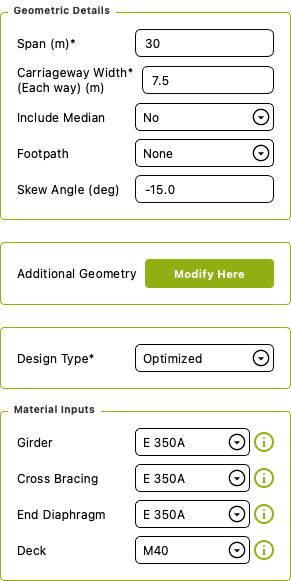
\includegraphics[width=0.30\linewidth]{../proofs/207_median_no_treated_as_yes/screenshots/03_after_clearing_carriageway_median_no.png}
\caption{Median = No; after the carriageway field is cleared it is reset to 7.5 (offscreen capture).}
\end{figure}

% ---- 208
\subsection{\issue{208} --- Design log never written to the PDF report}
\textbf{Severity / tier:} \sevM\ / T1. \quad \textbf{Proof:} \proof{208\_design\_log\_dropped\_from\_report/}

\textbf{Description.} \texttt{build\_report\_payload} (\texttt{report\_generator.py:770--792}) collects the design log and passes it to \texttt{ch8\_design\_log} (line 937). That function formats every INFO, WARNING and ERROR line into \texttt{lines\_tex}, then returns only the Standards \& Assumptions text (\texttt{chap8.py:38}).

\textbf{End-to-end evidence (two runs).} A full report was generated with three marker lines in \texttt{output\_dict['design\_log']}. The payload contained all three markers, and the generated \texttt{.tex} contained none of them. The complete report is included in the proof folder.

\textbf{Root cause:} \texttt{chap8.py:38} (introduced in commit \texttt{b6c0a10}). \quad \textbf{Fix (proven):} append the collected lines to the returned chapter.

% ---- 209
\subsection{\issue{209} --- \texttt{\_lookup\_material} returns \texttt{None}}
\textbf{Severity / tier:} \sevL\ / T1. \quad \textbf{Proof:} \proof{209\_lookup\_material\_returns\_none/}

\textbf{Description.} The function is annotated \texttt{-> float}, and its docstring promises a fallback. For a grade or property with no database row it returns \texttt{None}; for an empty name it raises \texttt{IndexError}. Its error message prints the class \texttt{sqlite3.Error} instead of the exception, and the connection is not closed when the query raises (\texttt{plategirderbridge.py:1124--1167}).

\textbf{Expected:} a float or a clear \texttt{LookupError}. \quad \textbf{Actual:} \texttt{None} / \texttt{IndexError}, identical in two processes.

% ---- 210
\subsection{\issue{210} --- Backslash in report text prints as ``\textbackslash\{\}''}
\textbf{Severity / tier:} \sevL\ / T1. \quad \textbf{Proof:} \proof{210\_tex\_backslash\_double\_escape/}

\textbf{Description.} \texttt{\_tex()} (\texttt{report\_utils.py:18--23}) escapes in sequential passes, so the braces of \texttt{\textbackslash textbackslash\{\}} are escaped again. For the project name \verb|A\textbf{B}| the generated source contains \verb|A\textbackslash\{\}textbf\{B\}|, which prints as ``A\textbackslash\{\}textbf\{B\}''. \textbf{Fix:} single-pass translation table.

\textbf{Security check (passed).} The project name \texttt{\textbackslash input\{/etc/hostname\}} is escaped, and the file is not read. \texttt{pdflatex} is called with a list of arguments, without a shell and without \texttt{-shell-escape}.

% ------------------------------------------------------------------ 8
\section{Contributions to existing issues}\label{sec:contrib}

\subsection{\issue{135} --- root cause of the second-\texttt{design()} crash}
\textbf{Proof:} \proof{135\_comment\_root\_cause\_double\_mm\_to\_m/}

\texttt{design()} calls \texttt{\_convert\_girder\_dims\_mm\_to\_m()} on every run (\texttt{plategirderbridge.py:683}). The function divides the values \emph{in} \texttt{self.input\_dict} by 1000 (lines 536--589).

\begin{center}\begin{tabular}{@{}ll@{}}
\toprule
State & Girder depth \texttt{G1.M1} \\
\midrule
After \texttt{set\_input} & 1670 (mm) \\
After run 1 & 1.67 (m, correct) \\
Run 2 & 0.00167 $\rightarrow$ \texttt{ValueError: math domain error} (LTB) \\
Run 2 with a pristine copy restored (fix proof) & 1.67, no crash \\
\bottomrule
\end{tabular}\end{center}
The desktop path calls \texttt{set\_input()} before every \texttt{design()} and did not crash for this input. The defect affects repeated use of the same object, for example a retry or a redesign.

\subsection{\issue{88} / \issue{180} --- non-finite values accepted}
\textbf{Proof:} \proof{088\_comment\_nan\_accepted\_by\_validators/}. Span, skew, carriageway and $f_y$ equal to NaN are accepted by \texttt{validate\_basic\_inputs} and \texttt{validate\_material\_inputs}, and \texttt{True} is accepted as a skew. \texttt{validate\_map\_coordinates} accepts latitude 999, \texttt{nan} and \texttt{inf}. Root cause: \texttt{\_to\_float} (\texttt{validator.py:1094--1097}).

\subsection{Root-cause detail contributed to existing issues (earlier sessions)}
\begin{longtable}{@{}p{2.6cm}p{5.4cm}p{3.2cm}p{4.2cm}@{}}
\toprule
Finding & Statement & Existing issue & Root cause located \\
\midrule
F1 & NaN span accepted by validator & \#88 & \texttt{\_to\_float} (validator.py L1094) returns NaN unchecked; both boundary comparisons (L32--35) are False for NaN \\
F2 & custom steel density never read by design pipeline & \#20 & \texttt{\_build\_material\_props} (plategirderbridge.py L1177) falls back to 78500\,N/m$^3$; key only read by the PDF report (chap3.py L280) \\
F4 & custom material values wiped at Design after OSI load & \#19 & priming with empty \texttt{\_material\_custom\_fields} re-exports empty fields; \texttt{\_update\_input\_dict} (input\_dock.py L1029) stores \texttt{None} \\
--- & default grade E 350A crashes at Stage 5 (``Gs not set'') & \#42 & \texttt{BridgeConfig.from\_plate\_girder\_bridge} (designer.py L309--315) reads \texttt{material.girder.g} which priming fills only for grades found in the DB \\
--- & missing \texttt{thermal\_load} case warnings during load combinations & \#92 & analyser.py L2576 warnings observed in the headless probe log \\
\bottomrule
\end{longtable}


% ------------------------------------------------------------------ 9
\section{Findings filed earlier (\issue{96} -- \issue{155})}
The following subsections are reproduced from version 1 of this report without changes to their technical content.

\subsection{\#96 --- .osi loader skips all custom-material validation}
\textbf{Link:} \url{https://github.com/Nidhikhare12/OsdagBridge/issues/96}

\textbf{Statement.} The \texttt{.osi} load path validates geometry and additional inputs, but no \texttt{material.*} key is ever validated, so a hand-edited file can carry e.g.\ \texttt{Fy\,=\,99999\,MPa} and load with ``Loaded OSI Successfully!''.

\textbf{Evidence (executed 2026-11-15, twice).}
\begin{verbatim}
validate_osi_inputs({'material.girder.fy': 99999.0,
                     'material.girder.density': 5.0,
                     'material.deck.fck': -3.0})
  -> is_valid = True, errors = []

BridgeInputValidator.validate_material_inputs (the check the
loader never calls) rejects all three:
  fy 99999  -> corrected to 1200.0
  density 5 -> corrected to 50.0
  fck -3    -> corrected to 10.0
\end{verbatim}

\textbf{Root cause.} \texttt{osi\_validator.py}: \texttt{\_BASIC\_KEYS} (L82--86) holds only span/carriageway/skew; \texttt{\_ADDITIONAL\_KEYS} (L89--111) holds many numeric limits but no \texttt{material.*} keys; \texttt{validate()} (L142--157) iterates only those lists, so \texttt{validate\_material\_inputs} --- the check the live Material Properties dialog enforces --- is unreachable from the load path (\texttt{template\_page.py} \texttt{loadOSI\_inputs} L847).

\textbf{Suggested fix (diff posted in the issue).} add the material keys to the OSI validation loop and route them through \texttt{validate\_material\_inputs} in \texttt{validate()}.

\subsection{\#97 --- input lock can crash when Additional Inputs dialog was never opened (T3, static)}
\textbf{Link:} \url{https://github.com/Nidhikhare12/OsdagBridge/issues/97}

\textbf{Statement.} Lock/unlock propagates state to the Additional Inputs dialog, but \texttt{InputDock.toggle\_lock()} dereferences the dialog without checking whether it has been instantiated; because the dialog is created lazily, toggling lock before opening Additional Inputs can raise \texttt{AttributeError} on \texttt{None}. (Reported as a T3 static finding from code reading; not executed as a runtime repro in this session.)

\textbf{Evidence (read-only, file:line).} \texttt{input\_dock.py:856--859} calls \texttt{self.parent.\_additional\_inputs\_dialog.lock(...)} unconditionally, while \texttt{template\_page.py:124} initializes \texttt{\_additional\_inputs\_dialog = None} and creates it on demand (\texttt{\_get\_additional\_inputs()}, L440--447); other call sites guard with \texttt{is not None} (e.g.\ L454,615,862).

\textbf{Suggested fix (diff posted in the issue).} guard the dereference, e.g. \texttt{dlg = getattr(self.parent, "\_additional\_inputs\_dialog", None)} then call \texttt{dlg.lock(...)} only if not \texttt{None}.

\subsection{\#98 --- \texttt{osdag\_core} metadata declares bogus \texttt{sqlite} dependency (T5)}
\textbf{Link:} \url{https://github.com/Nidhikhare12/OsdagBridge/issues/98}

\textbf{Statement.} The installed \texttt{osdag\_core 0.0.0} package used with OsdagBridge declares \texttt{sqlite} in its \texttt{Requires-Dist} metadata. \texttt{sqlite} is not a valid/installable PyPI distribution for the stdlib module (\texttt{sqlite3}); this can break dependency resolution in clean environments.

\textbf{Evidence.} \texttt{importlib.metadata.distribution("osdag\_core").metadata.get\_all("Requires-Dist")} includes \texttt{'sqlite'} (recorded in \texttt{evidence/logs/phase1\_installed\_meta.txt}); \texttt{tests/test\_phase1\_packaging.py::test\_osdag\_core\_declares\_bogus\_sqlite\_dep} confirms it.

\textbf{Suggested fix (posted in the issue).} remove \texttt{sqlite} from \texttt{osdag\_core} \texttt{Requires-Dist} (stdlib \texttt{sqlite3} needs no pip dependency) or reference a corrected build in OsdagBridge setup.

\subsection{\#99 --- \texttt{pyproject.toml} runtime dependencies omit required packages and declare unused \texttt{pydantic} (T5)}
\textbf{Link:} \url{https://github.com/Nidhikhare12/OsdagBridge/issues/99}

\textbf{Statement.} \texttt{pyproject.toml} declares \texttt{[scipy,fiona,shapely,pydantic,matplotlib,openseespy,opsvis,xarray]} but omits packages directly imported/used in source (e.g.\ \texttt{PySide6}, \texttt{numpy}, \texttt{osdag\_core}, \texttt{yaml} usage at \texttt{template\_page.py:812,839}, \texttt{navcube}, \texttt{OCC}, \texttt{plotly}, \texttt{ifcopenshell}, \texttt{openpyxl}, \texttt{pandas}), while \texttt{pydantic} has no observed imports in \texttt{src}. With \texttt{README} instructing \texttt{pip install -e .}, affected features can fail in fresh installs.

\textbf{Evidence.} Import/usage proof in \texttt{evidence/logs/phase1\_imports\_clean.txt} and \texttt{evidence/logs/phase1\_p1\_002\_proof.txt}; \texttt{tests/test\_phase1\_packaging.py::test\_pyproject\_missing\_key\_runtime\_deps}.

\textbf{Suggested fix (posted in the issue).} add missing runtime deps and/or optional extras to match actual requirements, reconcile \texttt{pydantic}, and align manifests/README.

\subsection{\#100 --- inconsistent dependency declarations across manifests (T6)}
\textbf{Link:} \url{https://github.com/Nidhikhare12/OsdagBridge/issues/100}

\textbf{Statement.} \texttt{pyproject.toml}, \texttt{requirements.txt}, and \texttt{environment.yml} declare different package sets (e.g.\ \texttt{PySide6/numpy/ifcopenshell/openpyxl} present in requirements but not in pyproject deps; \texttt{matplotlib/openseespy/opsvis} differ; env relies on \texttt{osdag::osdag} and \texttt{-e .}), creating conflicting install guidance.

\textbf{Evidence.} Manifests read from \texttt{dev @ d74f56d}; compared against actual imports/usage (\texttt{evidence/logs/phase1\_*}).

\textbf{Suggested fix (posted in the issue).} establish a single source of truth (e.g.\ \texttt{pyproject} + extras), align/generate other manifests, and document per-workflow install paths.

\subsection{\#101 --- README documents CLI usage but CLI entrypoint is a stub that ignores arguments (T6)}
\textbf{Link:} \url{https://github.com/Nidhikhare12/OsdagBridge/issues/101}

\textbf{Statement.} \texttt{README.md} presents CLI support and documents example commands (e.g.\ \texttt{osdagbridge analyze project.yaml --solver native}, \texttt{osdagbridge report project.yaml report.pdf}), but the installed console script \texttt{osdagbridge-cli} (\texttt{pyproject.toml:85}) resolves to \texttt{osdagbridge.cli.\_\_main\_\_.main} which only prints \texttt{"osdagbridge CLI (stub)"} and ignores all arguments including \texttt{--help}.

\textbf{Evidence.} \texttt{README.md:4,18,102,108,154}; \texttt{src/osdagbridge/cli/\_\_main\_\_.py} stub; invocations recorded in \texttt{evidence/logs/phase1\_entrypoints.txt}; \texttt{tests/test\_phase1\_packaging.py::test\_cli\_stub\_ignores\_args}.

\textbf{Suggested fix (posted in the issue).} implement argument parsing and documented commands, or clearly mark CLI as unimplemented/WIP in README and align documented vs installed command names.

\subsection{\#127 --- verification example YAMLs are empty placeholders that fail validation (T6)}
\textbf{Link:} \url{https://github.com/Nidhikhare12/OsdagBridge/issues/127}

\textbf{Statement.} \texttt{examples/plate\_girder/verification\_case\_01.yaml} and \texttt{verification\_case\_02.yaml} are empty/comment-only placeholders (no valid input dictionary) and fail \texttt{validate\_osi\_inputs}.

\textbf{Evidence.} \texttt{evidence/logs/phase1\_examples.txt}: both load as \texttt{None}/no keys with \texttt{is\_valid=False}, error \texttt{['File does not contain a valid input dictionary.']}; \texttt{tests/test\_phase1\_packaging.py::test\_examples\_parse\_and\_validate}.

\textbf{Suggested fix (posted in the issue).} populate with valid representative inputs that pass validation, or clearly mark/exclude as placeholders.

\subsection{\#128 --- \texttt{example\_basic.yaml} uses placeholder keys but passes validation vacuously (T7)}
\textbf{Link:} \url{https://github.com/Nidhikhare12/OsdagBridge/issues/128}

\textbf{Statement.} \texttt{examples/plate\_girder/example\_basic.yaml} uses a placeholder schema (e.g.\ \texttt{project.span\_m}) with no real dotted OSI keys (e.g.\ \texttt{geometry.span}), yet \texttt{validate\_osi\_inputs} returns \texttt{is\_valid=True} with no errors/warnings because it polices only present known keys.

\textbf{Evidence.} \texttt{evidence/logs/phase1\_examples.txt}: top-level \texttt{['project']}, no real span/cw/skew dotted keys, \texttt{validate.is\_valid=True}; \texttt{tests/test\_phase1\_packaging.py::test\_examples\_parse\_and\_validate}.

\textbf{Suggested fix (posted in the issue).} provide real OSI-key example values, or clearly mark as a non-loadable placeholder/template.

\subsection{\#129 --- \texttt{validate\_material\_inputs} skips range checks for cross-bracing/end-diaphragm material keys (T2)}
\textbf{Link:} \url{https://github.com/Nidhikhare12/OsdagBridge/issues/129}

\textbf{Statement.} \texttt{BridgeInputValidator.validate\_material\_inputs} enforces per-field ranges for girder/deck material keys but has no branches for \texttt{material.cross\_bracing.*} or \texttt{material.end\_diaphragm.*}, so out-of-range CB/ED custom material values are accepted.

\textbf{Evidence.} Executed calls in \texttt{scripts/drift\_check.py} (\texttt{evidence/logs/phase3\_drift\_check.txt}): girder Fy=5000 rejected; cross-bracing/end-diaphragm Fy=5000 and sampled Fu/E/density extremes accepted (returned \texttt{None}). Code: \texttt{validator.py} $\approx$L78--172 handles only girder/deck keys.

\textbf{Suggested fix (posted in the issue).} extend per-field validation to CB/ED steel material keys (same/component-appropriate ranges) or explicitly handle/flag them.

\subsection{\#130 --- integer validators raise \texttt{OverflowError} on \texttt{inf}/\texttt{-inf} instead of a validation message (T2)}
\textbf{Link:} \url{https://github.com/Nidhikhare12/OsdagBridge/issues/130}

\textbf{Statement.} \texttt{BridgeInputValidator.validate\_additional\_inputs} raises \texttt{OverflowError: cannot convert float infinity to integer} for \texttt{inf}/\texttt{-inf} on several integer fields instead of returning a validation correction/message.

\textbf{Evidence.} Executed fuzz (\texttt{scripts/validator\_fuzz.py}, \texttt{evidence/logs/trackF\_validator\_fuzz.*}): 10 exceptions for \texttt{KEY\_TS\_NO\_OF\_GIRDERS}, \texttt{KEY\_WC\_LD\_LANE\_TABLE\_COUNT}, \texttt{KEY\_MP\_CB\_NO\_OF\_CROSS\_BRACINGS}, \texttt{KEY\_DS\_STUD\_COUNT}, \texttt{KEY\_DO\_LOAD\_CYCLES}.

\textbf{Suggested fix (posted in the issue).} reject non-finite values before integer conversion (e.g. in \texttt{\_to\_int}) and return an appropriate validation message.

\subsection{\#131 --- \texttt{saveOSI\_inputs} uses \texttt{yaml.dump} unsafe tags incompatible with \texttt{yaml.safe\_load} (T2)}
\textbf{Link:} \url{https://github.com/Nidhikhare12/OsdagBridge/issues/131}

\textbf{Statement.} \texttt{saveOSI\_inputs} writes with \texttt{yaml.dump} while \texttt{loadOSI\_inputs} reads with \texttt{yaml.safe\_load}; unsafe Python tags (e.g. numpy scalars, tuples, sets) can be saved but fail to load.

\textbf{Evidence.} Executed YAML round-trip (\texttt{evidence/logs/trackI\_yaml\_dump\_safe\_load.txt}): dump of dict containing \texttt{np.float64}, tuple, set produces \texttt{!!python/...}/\texttt{!!set}/\texttt{!!python/tuple} tags and \texttt{yaml.safe\_load} raises \texttt{ConstructorError}. Code: \texttt{template\_page.py} $\approx$793--850.

\textbf{Suggested fix (posted in the issue).} use \texttt{yaml.safe\_dump} and/or normalize types (numpy scalars, tuples, sets) before saving for safe round-trip.

\subsection{\#132 --- skew sign is not mirror-symmetric (T2)}
\textbf{Link:} \url{https://github.com/Nidhikhare12/OsdagBridge/issues/132}

\textbf{Statement.} For a symmetric section (no median/footpath), flipping skew sign mirrors the bridge; demands should match. Executed headless designs (span 30, cw 10.5, Optimized) show +15° vs -15°: \texttt{util.shear} 59.28 vs 41.08, \texttt{util.fatigue} 183.74 vs 167.06; +7.5° vs -7.5°: 62.32 vs 42.18, 182.25 vs 175.33 — while self-weight checks are identical. Sign of a symmetric parameter changes the design.

\textbf{Evidence.} \texttt{dictionaries/OR\_SKEW\{15,M15,75,M75\}/output.json}, \texttt{evidence/logs/oracle\_runs\{1,2\}.log}; scripts \texttt{oracle\_runs.py}, \texttt{design\_runner.py}.

\textbf{Suggested fix (posted in the issue).} make live-load placement / oblique-mesh load mapping mirror-invariant; regression test that DCR magnitudes for positive and negative skew match within tolerance.

\subsection{\#133 --- \texttt{design()} non-termination on valid span-45 + median + footpath inputs (T2)}
\textbf{Link:} \url{https://github.com/Nidhikhare12/OsdagBridge/issues/133}

\textbf{Statement.} Valid in-limits inputs (span 45 m, cw 15 m, median Yes, footpaths) make \texttt{design()} exceed 600 s without producing output; a no-timeout rerun consumed $>12$ min CPU with no result. Control cases complete in 28--261 s. Non-convergent \texttt{fsolve} warnings appear in the case logs.

\textbf{Evidence.} \texttt{evidence/logs/design\_sweep\_run.log} (SW03/SW06 timeout), \texttt{evidence/logs/SW03\_rerun.log}, \texttt{dictionaries/SW03/case.log}, controls \texttt{dictionaries/OR\_SPAN45/result.json}.

\textbf{Suggested fix (posted in the issue).} bound the moving-load/envelope solver so non-convergent cases terminate with a clear warning; add a regression test with a time budget.

\subsection{\#134 --- wrong PASS: silent live-load skip gives zero ULS demand (T1)}
\textbf{Link:} \url{https://github.com/Nidhikhare12/OsdagBridge/issues/134}

\textbf{Statement.} Valid inputs (span 30, cw 7.5, skew 0, footpath Both Sides, median Yes) make governing-LL detection fail (\texttt{analyser.py:1998} warning); no live-load case is created, \texttt{mu\_applied=0.0}, all structural DCRs $=0$, yet the design reports \texttt{Status PASS}. Four near-neighbor controls (one field changed) show normal nonzero demands.

\textbf{Evidence.} \texttt{dictionaries/SW05/case.log}, \texttt{dictionaries/P5\_SW05R/run.log}, \texttt{dictionaries/P5\_SW05R/output.json}; controls \texttt{dictionaries/P5\_MED\_NOFOOT}, \texttt{P5\_FOOT\_NOMED}, \texttt{P5\_MED\_CW105}.

\textbf{Suggested fix (posted in the issue).} use \texttt{method="nearest"} on the \texttt{Element} lookup and/or raise on governing-LL detection failure instead of continuing to PASS.

\subsection{\#135 --- second \texttt{design()} on same object crashes in LTB buckling (T1)}
\textbf{Link:} \url{https://github.com/Nidhikhare12/OsdagBridge/issues/135}

\textbf{Statement.} Calling \texttt{design()} twice on the same \texttt{PlateGirderBridge} object: run 1 completes, run 2 crashes with \texttt{ValueError: math domain error} in \texttt{irc22\_2015.py:639} (\texttt{math.sqrt(beta\_b*(Zp*fy)/Mcr)}), stage 5 LTB check — stale per-run state. No duplicate (\#85 is CAD-display on 2nd run, no crash).

\textbf{Evidence.} guarded harness \texttt{dictionaries/IDEM2/same.py}; \texttt{evidence/logs/determinism\_2.log} (RUN1\_DONE then ValueError); full traceback \texttt{dictionaries/IDEM2/same.log}. An unguarded earlier harness (forkserver re-exec) was discarded as an artifact.

\textbf{Suggested fix (posted in the issue).} reset all per-run section/DTO state at the start of \texttt{design()}, guard the LTB sqrt, and add an idempotence regression test.

\subsection{\#153 --- \texttt{saveOSI\_inputs} does not enforce the .osi file extension (T3)}
\textbf{Link:} \url{https://github.com/Nidhikhare12/OsdagBridge/issues/153}

\textbf{Statement.} In \texttt{saveOSI\_inputs()} (\texttt{desktop/ui/template\_page.py:793--826}), the path returned by \texttt{QFileDialog.getSaveFileName(self, ``Save Design Inputs'', default\_dir, ``Input Files(*.osi)'', None)} is passed unmodified to \texttt{open(filePath, 'w')}. Nothing checks or appends the \texttt{.osi} extension, so a user typing \texttt{my\_design.txt} saves a file that the loader's \texttt{*.osi} filter will not list. A plain rename is required before the file can be loaded.

\textbf{Evidence.} \texttt{notes/osi\_load\_path.md} (OSI save/load path analysis, STEP 2); \texttt{template\_page.py:802--806} (dialog), \texttt{template\_page.py:812} (\texttt{open(filePath, 'w')}); we recorded the finding as \textbf{P6-015} (T3, static) on 2026-11-18 in \texttt{notes/all\_issues\_and\_bugs.md}. The identical review (same file/lines, same fix) was filed upstream as \#153 (2026-11-18); P6-015 was reclassified to T4 duplicate. Comment draft: \texttt{notes/issue\_drafts/25\_comment\_153\_osi\_extension\_t4.md}.

\textbf{Expected vs actual.} \emph{Expected:} \texttt{.osi} appended automatically or a warning shown. \emph{Actual:} any filename accepted; no enforcement, no warning.

\textbf{Suggested fix (as filed in the issue).} \texttt{if not filePath.lower().endswith(".osi"): filePath += ".osi"} before \texttt{open(...)}; or display a warning for unsupported extensions.

\textbf{Severity / confidence.} S3 (usability; the saved file is invisible to the load filter) / High (static, path unambiguous).

\subsection{\#154 --- \texttt{loadOSI\_inputs} silently swallows exceptions from \texttt{solve\_extend\_basic\_input\_dict} (T3)}
\textbf{Link:} \url{https://github.com/Nidhikhare12/OsdagBridge/issues/154}

\textbf{Statement.} In \texttt{loadOSI\_inputs()}, the order is: (1) \texttt{validate\_osi\_inputs(data)}; (2) on success, \texttt{populate\_from\_dict(data)} populates the dock; (3) \texttt{solve\_extend\_basic\_input\_dict(self.input\_dict)} runs inside a bare \texttt{try/except Exception: pass}. Any exception raised by the solve step --- invalid material values that slipped through validation, or any arithmetic failure --- is swallowed with no log and no message. The UI is left showing the loaded values even though the solver rejected them.

\textbf{Evidence.} \texttt{notes/osi\_load\_path.md} (item 4: exceptions silently swallowed); \texttt{template\_page.py:847--870} (validate $\rightarrow$ populate $\rightarrow$ \texttt{except Exception: pass}); recorded as \textbf{P6-017} (T3, static) on 2026-11-18 in \texttt{notes/all\_issues\_and\_bugs.md}. The identical review (same code path) was filed upstream as \#154 (2026-11-18); P6-017 was reclassified to T4 duplicate. Comment draft: \texttt{notes/issue\_drafts/26\_comment\_154\_osi\_swallow\_t4.md}.

\textbf{Expected vs actual.} \emph{Expected:} the solve failure surfaces an error to the user and the load aborts (or the dock is not populated). \emph{Actual:} the exception disappears; the dock shows the loaded values as if the load succeeded.

\textbf{Suggested fix (as filed in the issue).} Catch the exception explicitly and surface it (e.g. \texttt{CustomMessageBox} error), preserving diagnostics and keeping UI/internal state consistent, instead of \texttt{pass}.

\textbf{Severity / confidence.} S2 (wrong data shown as if load succeeded) / High (static, code path unambiguous).

\subsection{\#155 --- web application layer absent (stub-only \texttt{web/}; T5/T6)}
\textbf{Link:} \url{https://github.com/Nidhikhare12/OsdagBridge/issues/155}

\textbf{Statement.} The 2026-11-18 GATE 0 inventory found that the OsdagBridge repository contains no runnable web application: no Django backend, no React frontend, and no HTTP API. The repository is a desktop application (PySide; UI in \texttt{desktop/ui/template\_page.py}) whose \texttt{web/} tree at the repository root contains only stubs. Web (Django/React) testing therefore cannot start; any documentation or task that assumes a web layer misstates the repository.

\textbf{Corrected repository-root inventory (read-only).}

\begin{longtable}{@{}p{5.2cm}p{5.6cm}p{4.2cm}@{}}
\toprule
Path / file & Content & Verdict \\
\midrule
\texttt{web/backend/manage.py} & \texttt{print("Django manage stub")} & stub --- no Django project \\
\texttt{web/frontend/package.json} & \texttt{\{"name":"osdagbridge-frontend","version":"0.0.0"\}} & stub --- no scripts / dependencies \\
\texttt{web/frontend/src/App.jsx} & \texttt{export default function App()\{ return null; \}} & placeholder --- renders nothing \\
\texttt{web/frontend/src/components/.gitkeep} & \texttt{\# placeholder} & intentionally empty \\
\texttt{web/.DS\_Store} & 6,148 bytes (macOS artifact) & noise \\
\bottomrule
\end{longtable}

No \texttt{settings.py}, \texttt{urls.py}, \texttt{wsgi.py}, models or views; no \texttt{urlpatterns} anywhere in the tree; no \texttt{fetch(}/\texttt{axios(} calls; no import of \texttt{osdagbridge.core} under \texttt{web/}. Note: \#155's evidence table lists the top-level \texttt{web/} directory as ``Not found'', which is inaccurate --- the directory exists but holds stubs; the conclusion (no usable web layer) is correct.

\textbf{Evidence.} \texttt{notes/web\_inventory.md} (corrected inventory); commands \texttt{find} under the clone's \texttt{web/} and \texttt{cat} of the four stub files; \texttt{grep -rn urlpatterns} (no matches). Recorded as \textbf{P1-007} (T9) in Phase 1; reclassified to T4 duplicate of \#155 on 2026-11-18. Comment draft: \texttt{notes/issue\_drafts/27\_comment\_155\_web\_layer\_absent\_t4.md}.

\textbf{Expected vs actual.} \emph{Expected:} a runnable Django + React layer, or documentation explicitly stating the desktop-only scope. \emph{Actual:} stub files only; no runnable app; web testing requires building one.

\textbf{Suggested resolution (as filed in the issue).} If web testing is in scope: implement the Django backend, React frontend and API integration. If the project is desktop-only: update README/requirements to describe desktop architecture and remove references to a non-existent web application. Testing-scope blocker --- not a defect in the desktop application.

\textbf{Severity / confidence.} Blocker (web testing only) / High (inventory reproducible; conclusion independent of path detail).


% ------------------------------------------------------------------ 10
\section{Static and security review}\label{sec:static}
\begin{longtable}{@{}L{4.6cm}L{6.6cm}L{4.6cm}@{}}
\toprule
Check & Result & Verdict \\
\midrule
\endhead
bandit (whole \texttt{src/osdagbridge}) & 0 high, 10 medium, 222 low; mostly \texttt{try/except/pass} (179) & T3, robustness only \\
ruff (F, B rules) & 2\,475 star-import uses, 226 unused imports, 23 call-in-default-argument & T3, code quality \\
pip-audit & No known vulnerabilities; local packages not auditable & T8 \\
\texttt{pdflatex} invocation & Argument list, no shell, no \texttt{-shell-escape}, temporary directory & T8 \\
LaTeX injection via project name & \texttt{\textbackslash input\{...\}} escaped, file not read & T8 \\
YAML handling & Load uses \texttt{safe\_load}; save uses \texttt{yaml.dump} & Known \issue{131} \\
\texttt{eval}/\texttt{exec} & Only in vendored \texttt{ospgrillage} on internally generated strings, plus GUI-only \texttt{exec} & T3, not reachable from user input \\
SQL & Table names interpolated from constants; values parameterised & T3 \\
\texttt{pickle}, \texttt{os.system}, \texttt{shell=True}, \texttt{mktemp} & No occurrences & T8 \\
\bottomrule
\end{longtable}

% ------------------------------------------------------------------ 11
\section{Behaviour checked and found correct}
\begin{itemize}[nosep]
  \item Typing \texttt{nan}, \texttt{inf}, \texttt{1e999} or \texttt{30,5} into span, skew or carriageway: blocked by \texttt{QDoubleValidator} or corrected with a message.
  \item A CJK project name, special characters (\texttt{\% \$ \_ \{ \} \textasciitilde{} \textasciicircum{} \# \&}) and a file name with spaces all produce a PDF report.
  \item A file name starting with \texttt{\&} or \texttt{-}: generation fails, and \texttt{pdf\_path} is correctly returned as \texttt{None}.
  \item The carriageway width is defined per carriageway (UI label ``Each way''), so the overall width with a median ($2w + w_m + 2w_{cb}$) is consistent.
  \item Carriageway widths 4.25--7.50\,m (span 25\,m, with median): the live load is never zero; the step at about 5.3\,m (one to two lanes, 366 to 845\,kNm) matches the IRC lane rule.
  \item Every completed design output in the corner sweep is free of NaN/inf and negative dimensions, and has $0 < \chi_{LT} \le 1$.
\end{itemize}

% ------------------------------------------------------------------ 12
\section{Limitations and open items}\label{sec:limits}
\begin{itemize}[nosep]
  \item \textbf{Corner sweep (L4):} wide-carriageway designs take up to 8 minutes each, so the counts in Section~\ref{sec:coverage} reflect the state at the time of writing. Two cases with span 20\,m, carriageway 23.6\,m and a median exceeded the 600\,s limit. The first (skew $-15^\circ$, both footpaths) ran while a second design process was sharing the CPU. The second (skew $+15^\circ$, no footpath) was running when the tester stopped the invalid L5 run, which also terminated its worker processes. Neither timeout is therefore treated as a finding; both are being rerun alone.
  \item \textbf{Multi-run sequences (L5):} the first attempt was invalid because of a harness defect (missing \texttt{\_\_main\_\_} guard with the pipeline's multiprocessing pool). It has been fixed and will be rerun.
  \item \textbf{Deck-geometry edge case} (100\,mm deck with 75\,mm covers): not tested, because the harness rebuilt the inputs and overwrote the deck parameters (T9, harness defect).
  \item \textbf{Not executed:} 3D CAD rendering and plot widgets (an offscreen OpenGL context is not available), and the project-location map dialog.
  \item Report text was checked at the \LaTeX\ source level; no PDF-to-text tool was available in the environment.
\end{itemize}

% ------------------------------------------------------------------ appendix
\appendix
\section{Reproducing the findings}
Every proof folder contains a \texttt{README.md} with the exact command, the expected and actual results, and a table of evidence files.
\begin{verbatim}
source ~/miniconda3/etc/profile.d/conda.sh && conda activate osdagbridge-env
cd osdagbridge-testing-report
python proofs/207_median_no_treated_as_yes/scripts/probe_median_fix.py
\end{verbatim}

\section{Earlier test log (version 1)}
\begin{longtable}{@{}p{1.4cm}p{3.0cm}p{6.2cm}p{2.6cm}p{2.0cm}@{}}
\toprule
ID & Area & Parameters (exact) & Result & Evidence \\
\midrule
PYT-01 & validator steel & density 49.9/50/120/120.1; fy 99.9/100/1200/1200.1; fu, E, G, Poisson, thermal at both boundaries & PASS (7 params) & \texttt{tests/test\_validator\_limits.py} \\
PYT-02 & validator deck & density, fck, fctm, Ecm, thermal at both boundaries & PASS (5 params) & same \\
PYT-03 & validator geometry & span 19.9/45.1 corrected; carriageway 4.25/23.6 pass, 23.7 corrected; median+5.0 $\rightarrow$ 7.5; skew $\pm$15.1 corrected & PASS & same \\
PYT-04 & validator NaN & span = NaN & \textbf{NaN accepted} (dup \#88) & pytest failure + root cause \\
PYT-05 & OSI round trip & dict $\rightarrow$ \texttt{yaml.dump} $\rightarrow$ \texttt{safe\_load} $\rightarrow$ equality + validation & PASS & \texttt{tests/test\_osi\_round\_trip.py} \\
F3-96 & OSI material bypass & fy 99999 / density 5 / fck $-$3 through the loader vs.\ the dialog check & \textbf{BUG} $\rightarrow$ \#96 & \texttt{evidence/analyze/osi\_material\_bypass.txt} \\
P2-001 & lock/unlock flow & toggle lock before Additional Inputs opened (static: \texttt{input\_dock.py:856--859}, lazy \texttt{template\_page.py:124,440--447}) & \textbf{ISSUE (T3)} $\rightarrow$ \#97 & \texttt{notes/issue\_drafts/01...} \\
P1-001 & packaging/metadata & \texttt{osdag\_core 0.0.0} \texttt{Requires-Dist} includes bogus \texttt{sqlite} (not installable; stdlib is \texttt{sqlite3}) & \textbf{ISSUE (T5)} $\rightarrow$ \#98 & \texttt{evidence/logs/phase1\_installed\_meta.txt} \\
P1-002 & packaging/pyproject & missing runtime deps (e.g.\ \texttt{PySide6}, \texttt{numpy}, \texttt{osdag\_core}, \texttt{yaml}, \texttt{OCC}) and unused \texttt{pydantic} vs \texttt{src} imports & \textbf{ISSUE (T5)} $\rightarrow$ \#99 & \texttt{evidence/logs/phase1\_p1\_002\_proof.txt} \\
P1-003 & packaging/manifests & \texttt{pyproject.toml}, \texttt{requirements.txt}, \texttt{environment.yml} declare inconsistent dep sets & \textbf{ISSUE (T6)} $\rightarrow$ \#100 & manifests at \texttt{dev @ d74f56d} \\
P1-004 & docs/CLI & README documents CLI commands/support but \texttt{osdagbridge-cli} entrypoint is a stub ignoring args/\texttt{--help} & \textbf{ISSUE (T6)} $\rightarrow$ \#101 & \texttt{evidence/logs/phase1\_entrypoints.txt} \\
P1-005 & docs/examples & \texttt{verification\_case\_01/02.yaml} are empty placeholders (no valid input dict), fail validation & \textbf{ISSUE (T6)} $\rightarrow$ \#127 & \texttt{evidence/logs/phase1\_examples.txt} \\
P1-006 & docs/examples & \texttt{example\_basic.yaml} uses non-real keys but passes \texttt{validate\_osi\_inputs} vacuously & \textbf{ISSUE (T7)} $\rightarrow$ \#128 & \texttt{evidence/logs/phase1\_examples.txt} \\
P3-001 & validation/material & \texttt{validate\_material\_inputs} skips range checks for CB/ED material keys (girder/deck only) & \textbf{ISSUE (T2)} $\rightarrow$ \#129 & \texttt{evidence/logs/phase3\_drift\_check.txt} \\
P4F-001 & validation/type & integer validators raise \texttt{OverflowError} on \texttt{inf}/\texttt{-inf} (5 integer keys) instead of message & \textbf{ISSUE (T2)} $\rightarrow$ \#130 & \texttt{evidence/logs/trackF\_validator\_fuzz.txt} \\
P4I-001 & io/osi & \texttt{saveOSI\_inputs} uses \texttt{yaml.dump} unsafe tags incompatible with \texttt{yaml.safe\_load} (round-trip can fail) & \textbf{ISSUE (T2)} $\rightarrow$ \#131 & \texttt{evidence/logs/trackI\_yaml\_dump\_safe\_load.txt} \\
P5-004 & analysis/skew & skew sign not mirror-symmetric: positive vs negative skew give different design demands (2 pairs) & \textbf{ISSUE (T2)} $\rightarrow$ \#132 & \texttt{dictionaries/OR\_SKEW*/output.json} \\
P5-005 & analysis/performance & \texttt{design()} non-termination ($>$10 min) on valid span-45 + median + footpath inputs & \textbf{ISSUE (T2)} $\rightarrow$ \#133 & \texttt{evidence/logs/design\_sweep\_run.log} \\
P5-006 & analysis/wrong-PASS & silent live-load skip gives zero ULS demand but verdict PASS (cw7.5+median+both footpaths) & \textbf{ISSUE (T1)} $\rightarrow$ \#134 & \texttt{dictionaries/P5\_SW05R/output.json} \\
P5-007 & crash/idempotence & 2nd \texttt{design()} on same object crashes in LTB sqrt (\texttt{math domain error}) & \textbf{ISSUE (T1)} $\rightarrow$ \#135 & \texttt{evidence/logs/determinism\_2.log} \\
\bottomrule
\end{longtable}


\section{Repository layout}
\begin{tabular}{@{}lL{11.5cm}@{}}
\toprule
\texttt{proofs/} & One folder per issue or comment: README, scripts, logs, inputs, screenshots, generated reports \\
\texttt{report/} & This report (\texttt{report.tex}, \texttt{sections/}) and the compiled \texttt{report.pdf} \\
\texttt{scripts/} & Test harnesses: \texttt{xrun.py}, \texttt{triage.py}, \texttt{minimize.py}, probes, sweeps \\
\texttt{tests/} & pytest suites and the extreme-value case registry (\texttt{tests/extreme/}) \\
\texttt{test\_cases/} & Baseline and generated minimal inputs \\
\texttt{evidence/} & Raw logs, sweep results (\texttt{evidence/xrun/}) \\
\texttt{dictionaries/} & Input/output dictionaries of design runs \\
\texttt{notes/} & Bug report, candidate list, issue drafts, duplicate-check data, state \\
\texttt{test\_log.md} & Row-per-test log (ID, parameters, expected, actual, result, evidence) \\
\bottomrule
\end{tabular}

\end{document}
